\begin{tikzpicture}%
\begin{scope}
\clip (1, .5) -- (.8, 1) -- (.8, 7.1) -- (1.1, 7.1) -- (1.2, 7) -- (7.3, 7) -- (7.3, .5) -- cycle ;
\node[anchor=south west,inner sep=0] at (0,0) {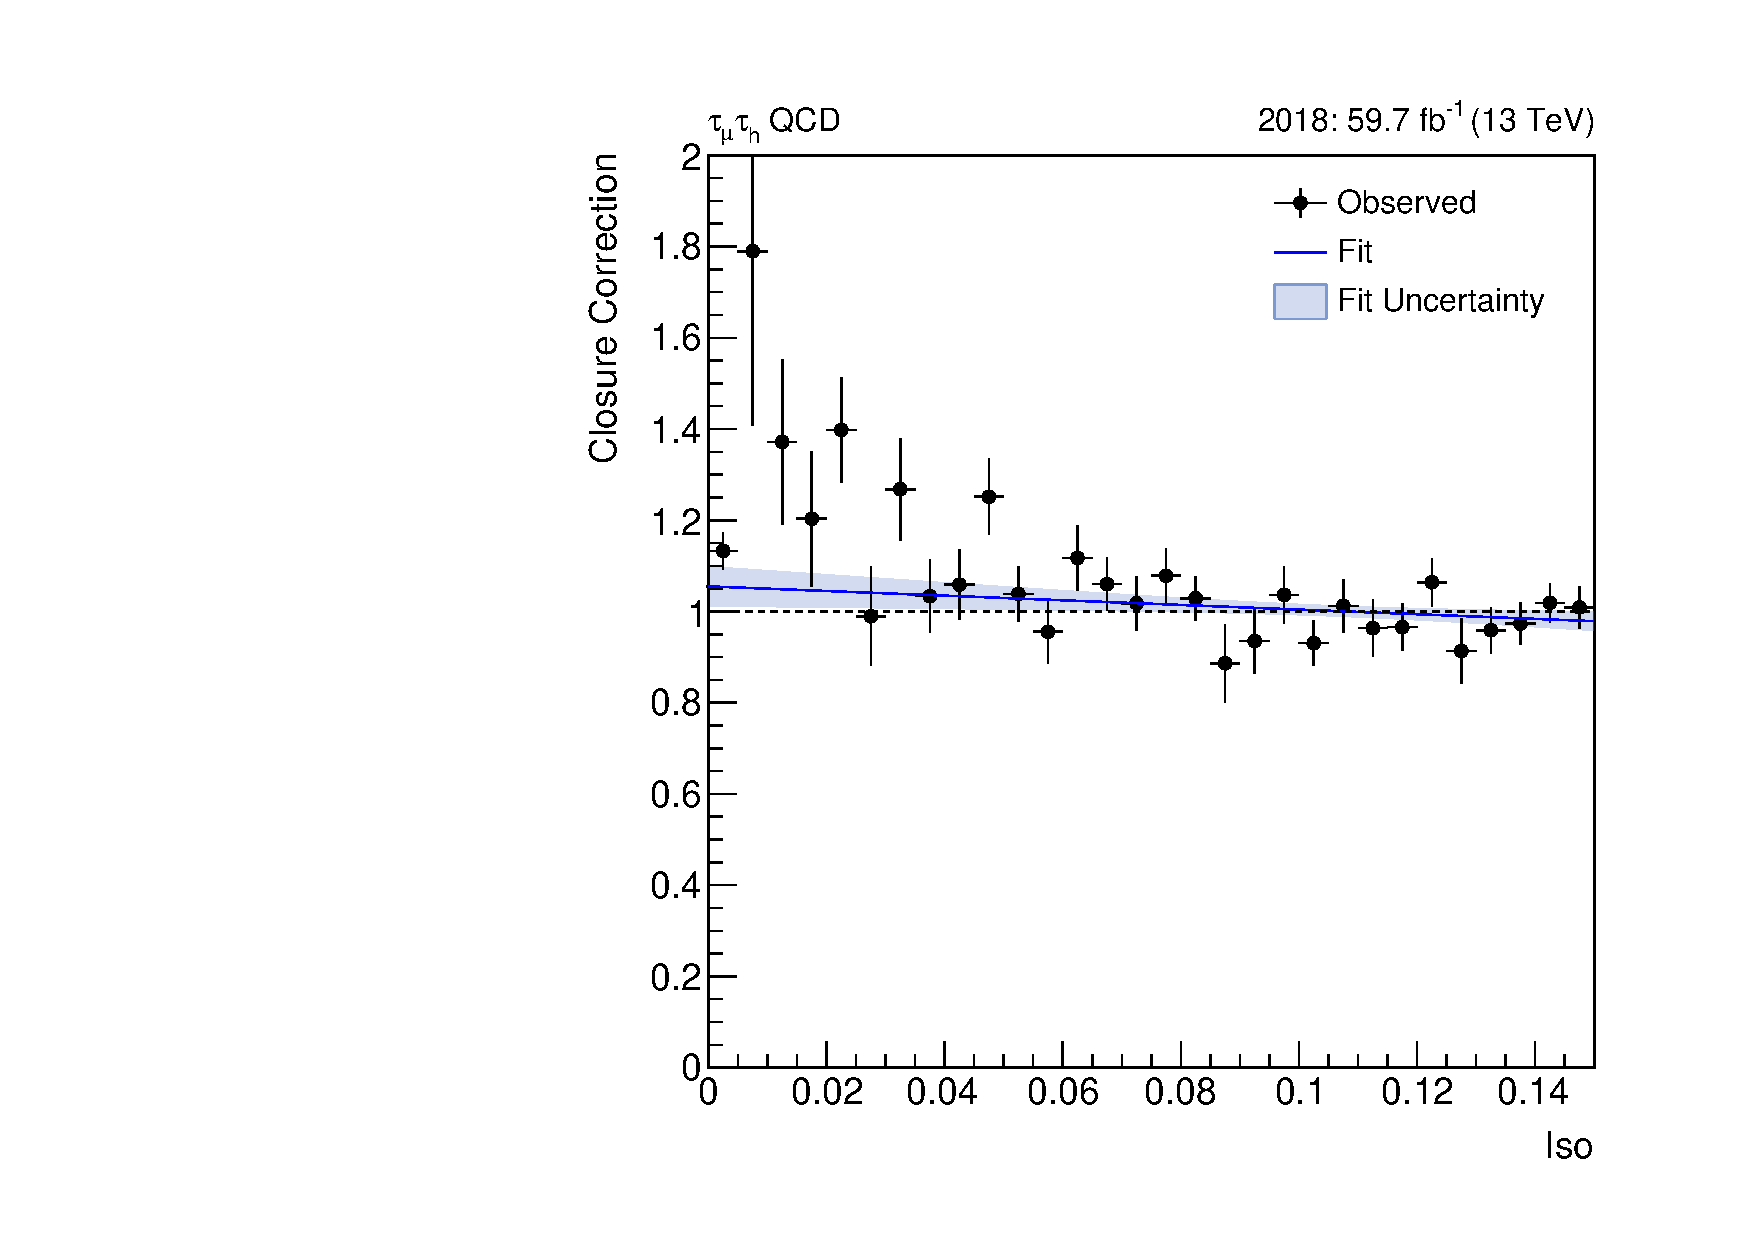
\includegraphics[width=8cm]{\PhDthesisdir/plots_and_images/from_CMS-NOTE-2020-218/ff_closure_iso_inclusive_closure_qcd_alt_mt_2018.pdf}};
\end{scope}

% year
\draw (7.35, 6.85) node [above left] {\scriptsize \SI{59.7}{\femto\barn^{-1}} (2018, \SI{13}{\TeV})\vphantom{Àq,}};

% category
\draw (1.1, 6.85) node [above right] {\scriptsize \mu\tauh, DR QCD};

% X axis label
\draw (7.2, -.1) node [above left] {\footnotesize $I_\text{rel}^{(\mu)}$\vphantom{Àq,}};

% Y axis label
\draw (.15, 7.2) node [below left, rotate=90] {\footnotesize Correction résiduelle sur $\FF_Q$\vphantom{Àq,}};

% CMS disclaimer
\draw (1.55, 1.65) node [below right] {\scriptsize CMS Data\vphantom{Àq,}};
\draw (3.55, 1.65) node [below right] {\scriptsize \WorkInProgress\vphantom{Àq,}};
\end{tikzpicture}